%%%%%%%%%%%%How does a GPS work and draw the state diagram for the GPS.Describe the different alternatives for measuring power consumption of a GPS%%%%%%%%%%%%%%%%%%%%%%%%%


\chapter{Background}



\subsection{GPS}
The Global positioning system is a space based radio navigation system developed by the Unites States Government.  The system provides both timing and geolocation information to a GPS receiver anywhere on the Earth.  The system is not influenced by the number of receivers and can therefore serve an unlimited amount of users. The GPS system can deliver a position which is accurate within 22 meters horizontally if only one receiver is used. If multiple receivers is used positioning accuracy level of the order of a subcentimeter to a few meters can be obtained \cite{GPS}.

GPS consists of 24 satellites that are arranged so that minimum four satellites is visible anywhere on the earth. Each satellite continuously broadcasts a signal composed of two carriers, two codes and a navigation message which contains the coordinates of the satellites.  If the distance between three satellites are known, the location of the receiver can be determined by measuring the angles with the respect of the each satellite.  Figure \ref{fig:GPS} shows the resection that is used by the satellites to determine the position.\\

\begin{minipage}[t]{0.8\textwidth}
\centering
    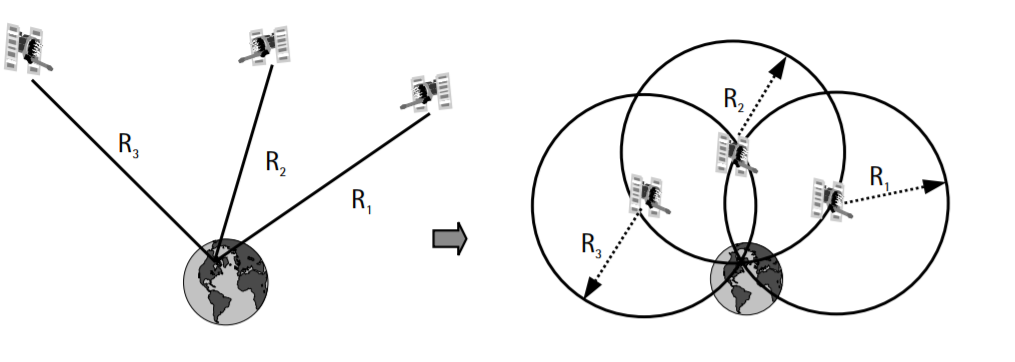
\includegraphics[width=0.8\textwidth]{Images/gps.PNG}\\
    \captionsetup{justification=centering}
    \captionof{figure}{Resection used by the satellites to determine the position}
    \label{fig:GPS}
\end{minipage}


  GPS needs an additional satellite to account for the clock offset. A method for determining the velocity of a GPS is by estimating the Doppler frequency of the received signal. The satellites broadcasts two types of navigation messages the Almanac and the Ephemeris. The Almanac contains course date for all the Space Vechicles(SV). Each SV broadcast this for ALL SVs. The Almanac is valid for up to several months. The Ephemeris contains precise information about orbital position and clock correction is only valid for up to 30 minutes. Both of these are critical for getting a GPS fix, and they are often one of the time limiting factor for getting the position. 
  An outdated almanac or ephemeris can cause a slow start, this can happen if the receiver hasn't been used in a while, a cold start is done or the receiver has traveled a far distance while turned off.
  
  A GPS reciever is often in of two states: Its

\subsection{Measurement methods}

There are several alternative for measuring the power consumption of a system. This section will give a brief summary of four methods, where three of them are circuit based and the fourth is software based. The circuit alternatives are heavily discussed and explained in \cite{Intersil},\cite{Infineon},\cite{Vishay}, while the software solution are based on Kadayif et al work 

\subsubsection{Shunt resistor}
A shunt resistor is often used to measure the energy consumption of a load because of its cost friendly and simple configuration. The shunt is placed in series with the device and the power supply.

If the voltage drop $V_{shunt}$ is measured, the current I can be calculated by Ohms law:\begin{equation}
V_{shunt}=R_{shunt}*I
\end{equation}

$R_{shunt}$ should be of a small value so it doesn't interference with the circuit. The power used by the device can then be calculated by using the power relation \begin{equation}
P=V_{load}*I \\
\end{equation}
\begin{equation}
V_{load}= V_{supply}-V_{shunt}
\end{equation}
\newline The resistor value of the shunt should be of a small value to minimize the power dissipated by the shunt. In \cite{Intersil} it is explained how the resistance value, temperature coefficient and the temperature resistance of the shunt resistor will affect the accuracy of the measurement:
\begin{equation}
\Delta R= R_{initial}* \Delta T * T_{coefficient}\\
\label{rchange}
\end{equation}
\begin{equation}
 \Delta T = \theta * I^{2}*R_{sense}
\end{equation}

The temperature change in the shunt comes mainly from the heat of the power dissipation that is caused by the current flowing into it. A smaller package has a higher thermal resistance $\theta$ and therefore a higher resistance change when power dissipation increases. Figure \ref{fig:Powererror} from \cite{Intersil} shows the error of three different shunt resistors with different packages. 

\begin{minipage}[t]{0.8\textwidth}
\centering
    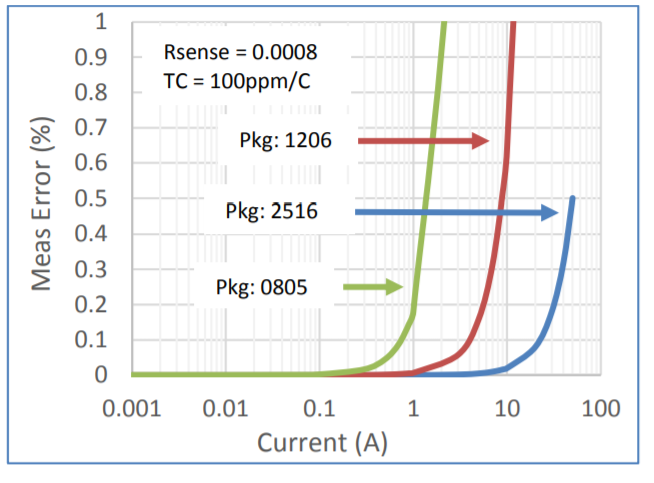
\includegraphics[width=0.8\textwidth]{Images/Powererror.PNG}\\
    \captionsetup{justification=centering}
    \captionof{figure}{The measurement error of three shunt resistors with different packages from \cite{Intersil}}
    \label{fig:Powererror}
\end{minipage}




The shunt can be placed either in a high side or low side configuration. A low-side shunt has one of its terminals grounded, this configuration might be preferable as the shunt resistor is not exposed of the high common node voltage that might had damage the measurement device. The configuration does also give the measurement device an easy access to common ground so that more signals can be measured at the same time in reference to a stable ground. A high-side configuration places the shunt between the power supply and the load. This might be preferable because it connects the load directly to the ground of the power supply. This configuration enables the shunt to detect leakages that appear before the load, which may have not been detected by the low-side configuration. Figure \ref{fig:shunt} shows the two configurations.

\begin{figure}[h]
\centering
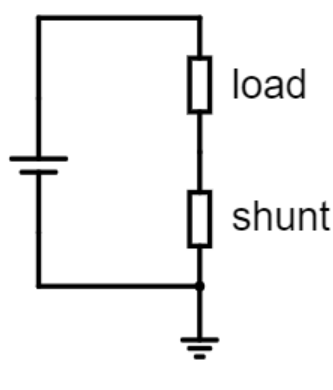
\includegraphics[height=4.5cm]{Project_Report/Images/shunt.PNG}
\caption{The setup for a low-side shunt and a high-side shunt to left and right respectively}
\label{fig:shunt}
\end{figure}



\subsubsection{DCR circuit}





\subsection{Hall effect}
The Hall effect can be exploited to measure the current in the circuit. When a current $I$ flows in to a conductor it also changes the magnitude of the magnetic field $H$ proportionately. The relation between the flux density $B$ and $I$ can be expressed as follows:


\begin{equation}
B= \mu_{0}*\mu_{r}*H= \dfrac{\mu{0}*\mu{r}*I}{2\pi r}
\end{equation}

An Hall effect IC consists of a Hall effect sensor which deliver an output signal which is a linear function with the flux density. The IC is a a loss less system because no resistance is inserted into the circuit and therefore a good method of sensing current without interfering the load.  The IC does also require a field concentrator to boost the flux density for the measurement.
\begin{figure}[h]
\centering
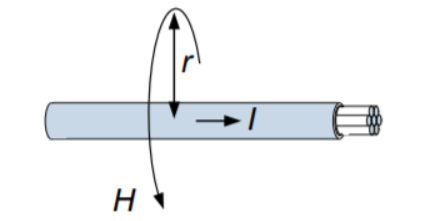
\includegraphics[height=4.5cm]{Project_Report/Images/current.PNG}
\caption{The induced magnetic field of a conductor from \cite{Infineon}}
\label{fig:current}
\end{figure}


\subsubsection{Code analysis}

The energy consumption of the GPS can be predicted by measuring each 